\documentclass[12pt]{article}
\usepackage{hyperref}
\usepackage{graphicx}
\graphicspath{{./}}
\usepackage{wrapfig}
\usepackage{dirtytalk}
\usepackage[table,xcdraw]{xcolor}
\usepackage{listings}
\usepackage{hyperref}
\usepackage{url}
\usepackage{pdfpages}
\usepackage{float}
\usepackage{mdframed}
\lstset{basicstyle=\small\ttfamily,
    columns=flexible,
    breaklines=true
}

\title{%
    GROOT: Infrastructure Security as a Service (ISaaS)\\
    \large Implementing Security Rules, Safeguards, and IPS tools for Private Cloud Infrastructures}


\author{Author \\
Aleksander Okonski \\
    aleksander.okonski.1656@student.uu.se \\
    aleksander.oko@gmail.com \\
    \vspace{2cm}
    \\
    Supervisor: Salman Toor \\
    Review: Bjorn Victor }
\date{}


\begin{document}
\maketitle
\newpage
\tableofcontents
\newpage

\section{Introduction}
The last several years, cloud computing has steadily grown (Figure \ref{fig:CloudTrendGoogle}) as a platform for businesses. Cloud computing is a term to describe computational resources that are located on a server running a software layer that disenfranchise the two. This allows for software to run independently of the hardware and allows a middle layer to control how the two interact. Cloud computing is not a new phenomenon\cite{rochwerger2009reservoir}.

\begin{figure}[ht]
    \centering
    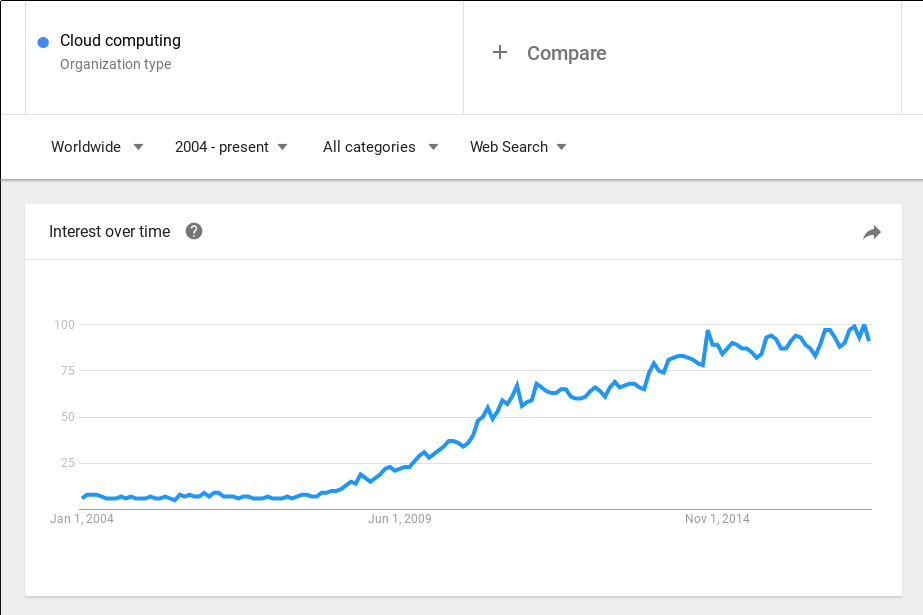
\includegraphics[scale=.3]{./pic/2017-06-14-130823_923x615_scrot.png}
    \caption{Cloud computing trend from Google Trends. Shows the interest in cloud computing between the years of 2004 to 2017. \cite{GoogleTrendsCloud}}
    \label{fig:CloudTrendGoogle}
\end{figure}

Cloud computing can be divided into 3 different categories: public, private, and hybrid.  The two main categories are public and private with the hybrid a mixture of the two. The later two are separated by two main categories, finances and physical location. Public clouds allow anyone to pay for the recourses that the individual would like to use. Therefore a user can spin up a virtual machine (VM) and then only pay for the amount of time that they use the resource. These VMs that a user spins up are usually hosted in data centers owned by the cloud provider. This means that the data the user puts onto the servers are stored on the cloud providers servers. The large players in this space are Amazon AWS \cite{amazonAWS} and Microsoft Azure \cite{Azure2017}. Private clouds typically only allow users of a particular organization to gain access the their recourses. Once the users gain access they may still need to pay for usage. The private clouds are simply more restrictive on who gains access the cloud resource. In addition private clouds are hosted on the organizations premise.  This means that the servers hosting the cloud are located in the organization and use the organizations network. This allows users to spin up VMs and have the data and computations happen on premise.

What the cloud provides to users ranges depending of the feature set of the cloud and the users needs. As a minimum, the cloud can typically create new virtual machines (VMs) that the user then has root access to. The users are then free to run any program they like. As cloud systems become more advanced with ever expanding user needs, more and more companies and individuals are migrating over to the cloud\cite{kondo2009cost}.

The year 2017 is shaping up to have some of the largest number of public attacks on computer systems \cite{newman_2017}. Cloud systems and the VMs that run on top of them are starting to be a major target for cyber criminals \cite{kellerman}. This transition to the cloud brings about new challenges, especially in the security space involving cloud systems. The users of the cloud spin up systems that have direct access to the Internet. These machines are susceptible to attacks especially with users not understanding the best practices in security \cite{ng2009studying,}. Users who configure software poorly lead to bugs and an expanded attack surface that then can be compromised.  Public cloud providers have created proprietary solutions to help mitigate having their users systems compromised. However private clouds do not have the manpower or funds to be able to tackle such a threat.

\iffalse
It is almost on a weekly bases that news of another security breach has effected a company \cite{newman_2017}.

\begin{figure}[ht]
    \centering
    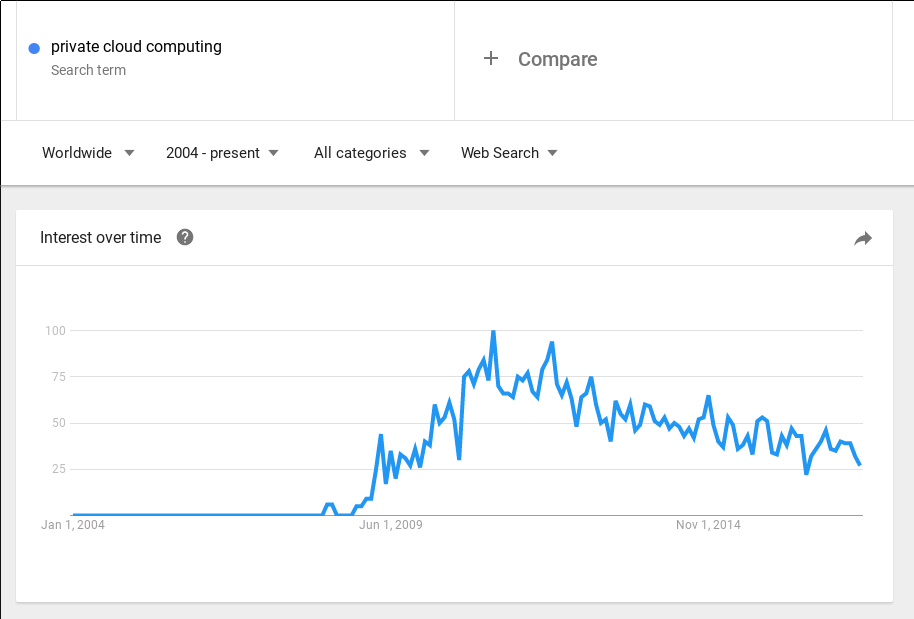
\includegraphics[scale=.3]{./pic/2017-06-14-135222_914x619_scrot.png}
    \caption{Private cloud computing trend from Google Trends. Shows the interest in private cloud computing between the years of 2004 to 2017. \cite{GoogleTrendsPriv}}
    \label{fig:PrivCloudTrendGoogle}
\end{figure}
\fi

The aim of this thesis is to facilitate security information in private cloud infrastructure when an organization does not have the resources to deploy sophisticated security solutions. Open source cloud solutions, such as OpenStack \cite{Openstack}, are becoming sought after solutions that allow anyone to create there own private cloud. These implementations lack a clear cut solution to security monitoring. This could lead to weaknesses being exploited in the private cloud allowing unauthorized users access to resources. To alleviate the threat a three step solution was created. The first was to create an outline that new users could follow to understand basic security practices when connecting to a VM. The second was to create an active monitoring solution within multi tenant environments. The solution is created to be versatile for any type of environment and for administrators to be able to obtain information with ease. Lastly a information gathering tool was created to obtain system data before termination of the infected resource. The project is designed to approach the security for private clouds actively instead of passively. The administrators should be able to detect vulnerabilities early before they are exploited. The proposed framework is a prototype solution that is able to identify vulnerabilities and report to administrators. These results were able to be used by administrators to prevent the vulnerability to be exploited.

\section{Background}
As can be seen in figure \ref{fig:CloudTrendGoogle}, cloud computing paradigm has gained a lot of attention over the last several years. Business and academia are looking at solutions to migrate their existing infrastructure to the cloud. There are several reasons for this type of business shift: costs, scalability, reliability \cite{DillonWuChang}. The cloud offers some precedented advantages to a standardized computational model. One is able to pay for only the resources used, with more resources added/removed depending on the demand. This is more commonly referred to as the pay-as-you-go-model. Another advantage is the ability to spin up/destroy several machines with little overhead. The usual use case for this is to scale up or down systems depending on the amount of work. Scaling can occurs in two was, vertical and horizontal scaling. Vertical scaling is when the VMs become larger; automatically add CPU, memory, and hard drive space. Horizontal scaling is when new machines are added to the cloud cluster to take on a larger work flow. Several companies are fronting the cloud revolution, some examples are Amazon\cite{amazonaws2017}, Google\cite{GoogleCloudCompute2017}, Microsoft\cite{Azure2017}, and Digital Ocean\cite{DigitalOcian2017}. These companies are providing a public cloud environment, that is to say that anyone can pay for computer resources. A user needs to sign up, provide a credit card, and then start setting up and launching whatever configuration of system they would like.
\begin{figure}[ht]
    \centering
    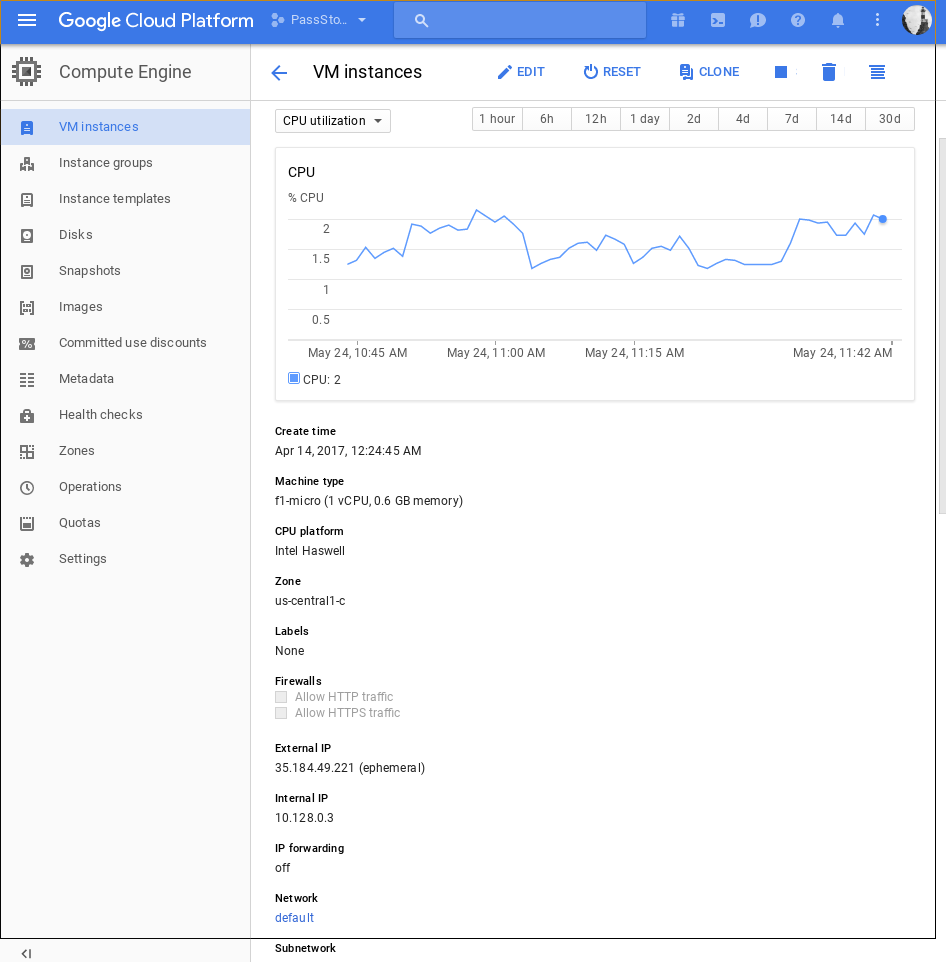
\includegraphics[scale=.2]{./pic/2017-05-24-114324_946x962_scrot.png}
    \caption{Google cloud interface for controlling VMs}
    \label{fig:GoogleInterface}
\end{figure}

The provider will then dedicate the specified hardware and allow the user to login that virtual machine and run whatever tasks the user would like to do. An example of the Google cloud compute engine is shown in figure \ref{fig:GoogleInterface}.  These public entities typically have teams dedicated to security and infrastructure monitoring. Have created proprietary solutions to ensure that the cloud environment \cite{SecAmazon} stay secure. As these security systems are a selling point for companies they are kept proprietary.

A private cloud is a different type of model where the cloud infrastructure is physically set inside a companies domain. Many companies would like to move over to a cloud based model but do not want to migrate there private resources into public domain. Therefor companies such as RackSpace, IBM, and VMware are providing private / hybrid cloud resources. This approach has part or the entire system built on site at the clients data center. This allows the client to hae most of the benefits of the cloud but also keep the system within there network. These clients typically don't have the recourses to create or manage a cloud security system.

\section{Problem Description}
In this work we will be looking at ways to protect VM clusters by ensuring proper configuration steps are setup and used with the addition of looking at ways to implement an intrusion prevention system (IPS) solution into the cloud environment. Security of computer systems is a large field. There are many different areas in the computer field and each one produces individual security challenges. For this project we focused on cloud infrastructure. Computer infrastructure exposed to the Internet face a large number of cyber attacks daily\cite{cimpanu_2017}. For private clouds this is ongoing problem as many of the users may not know of proper security protocols and leave ports such as SSH open. These types of security vulnerabilities would allow an attacker to gain full control of the virtual machines. To protect the public cloud, such as OpenStack, the mechanisms are thin. The administrators could attempt to monitor network traffic or install specific software on each VM. These solutions are either difficult to set up and maintain or only passively work. Network scanning does not prevent threats but tries to catch ongoing attacks \cite{global}. This may lead to vulnerabilities present in systems that the administrators do not know about. Its also impractical having to deploy a security solution to every VM that is started on the system. Users may not turn these systems on or may require different OS version that are not compatible with a security system. One of the benefits of the cloud is allowing users to set up and deploy computers with ease, adding additional factors may discourage users. Therefor the purpose of this project was to create an active system that can monitor other VMs for potential vulnerabilities. Users and administrators do not want to have systems taken over by malicious users that then perform actions like sending spam or stealing information. The created solution is able to identify vulnerabilities in VM configurations and alert the administrator's before the vulnerability is exploited.

\section{Related Work}
Before looking at cloud computing and security issues related to the specific field it is a good idea to look at what had been done to securing a standard server. A typical server would sit behind a firewall with an intrusion detection system (IDS) \cite{DigitalOcianServerSecurity} running alongside.  These systems would usually only be run by administrators who have had previous knowledge of how to maintain large Internet facing systems. One of the main goals in protecting these type of systems is to reduce attack surface. The firewall is used to filter traffic and ensure that only packets of a particular type are passed to the server while other packets were dropped. The IDS system would inspect traffic for malicious content and notify administrators if any was found. This model was a nice standard for how systems facing the Internet should be set up. However as users typically gain root access to the provisioned VMs it is much harder to have these types of machines sit behind a firewall and IDS. Different users may require different ports open that run different services, therefore a firewall would have to be configured for each user. \footnote{There is a side note to be said here, users can elect to create their own virtual firewall in the cloud. The users then can set up specific rules, this however tends to only occur when an entire on premise system is moved to the cloud and not when individual machines are set up.} This leads to many VMs being directly exposed to the Internet and attacks. Due to this cloud security had been a hot topic in recent times, therefor several papers have been written \cite{zissis2012addressing, mishra2013cloud, krutz2010cloud}. These particular papers focus on the different aspects and concerns that are present when running in a cloud environment. They are a nice starting point to look at how the threat landscape in the cloud differs from the standard model.

In addition important distinction between a centralized and cloud environment is how information is treated, a good article that describes this is "Addressing cloud computing security issues" \cite{zissis2012addressing}. The three staples of information security are confidentiality, integrity, and availability. In the cloud new difficulties come up for each of these classifications as data in the cloud may move around without the users knowledge.  The second set of articles  are looking at intrusion detection systems (IDS), more specifically how these can be used within the cloud \cite{SurveyOfIDS, patel2013intrusion}. These articles did not focus so much on implementation as they were focused more on the theory. An interesting comparison that shows the advantages and disadvantages for different IDS systems is presented table $2$ in "A survey of intrusion detection techniques in Cloud" \cite[SurveyOfIDS]. This is the basis for the types of IPS solutions that were chosen for this project. As this work was primarily focused on OpenStack, one particular IDS conference talk was used as a starting point for this research \cite{videoPresentation}.

The type of network and system monitoring that is proposed in this work is not new. At Cambridge University a set of probes are running on networks to ensure no security holes and ensure administrator's know what is running on the network \cite{CambUni}. In this research a similar type of probing was created for the OpenStack cloud platform.

\subsection{Open Source vs Closed Source}
Before getting into different aspects of cloud computing an important distinction to talk about is open source vs cloud source software. An open source project is a type of project that has the source code to the project freely available for any one to download, modify, and run. This allows a community of enthusiast's to support and expand the project. These projects can be very popular and can expand to a very large scale, some examples of popular projects are Linux \cite{Linux}, atom \cite{atom}, and FreeBSD \cite{freebsd}. Users contribute time in writing code, filling out documentation, or filing bugs this slowly expands the project. Goals for projects are laid out by the community, if a user does not agree with a decision they are allowed to fork a project and take it in a direction that they choose.  Typical projects are founded through donations or through the time of users.  A closed source coding projects is typically found in corporations. The code is not typically available and only the end product is distributed to consumers. The project goals are outlined to fit into a release time line. Full time workers then will work on the project to meet these deadlines. There typically is funding available for these types of projects with the end product monetized for profit.

\subsection{Cloud Models}
As mentioned above the cloud space consists of three types of clouds: public, hybrid, and private. The public cloud enables anyone to connect to the host and set up a machine. The host machines that run the cloud environment are located in public data centers throughout the world. The virtual machines are created then run and can be connected to the Internet. The public cloud typically runs on a model called pay as you go. This means that a user is charged for every hour of runtime or anther metric. The private cloud consist of the host being located in a private hosting environment. The virtual machines that are created are collocated on the internal network. The hybrid environment merges the two, with having some of the machines collocated in private data centers and others located on public data centers. Each of these models have benefits and drawbacks and have to evaluated for each individual project. The these cloud models all share a smiler set of tools employed to provide the necessary computational recourses to users.

In the cloud computing space several computational models exist \cite{neto2011demystifying}. These models reflect the different stages of a computer: hardware (Software as a Service), operating system (Platform as a Service), and software (Software as a Service).

\begin{itemize}
    \item Infrastructure as a Service (IaaS) gives the users a basic virtual machine with the user needing to set up all necessary functionality. This moves the responsibility of management of the hardware, network, and storage from the user to the operator. For the cloud IaaS build the back bone for the other modules to be built off of.

        Infrastructure is the bases of all systems, before cloud computing this was typically server and networking components. Microsoft gives a good explanation bellow:
        "The capability provided to the consumer is to provision processing, storage, networks, and other fundamental computing resources where the consumer is able to deploy and run arbitrary software, which can include operating systems and applications. The consumer does not manage or control the underlying cloud physical infrastructure but has control over operating systems, storage, deployed applications, and possibly limited control of select networking components." \cite{TechWikiMic}

    \item Platform as a Service (PaaS) give the user the ability to create applications (I.E. Web servers, databases, etc.) without the need to create the entire system from the ground up. The PaaS build from the IaaS and utilizes the hardware of IaaS to provide the users the platform that they desire.

        Platform software is a layer of software that enables a user to build their own software from. Some examples of this are the Apache web framework, wordpress, and mysql. A user can install Apache onto their server to create a website. With the cloud model a user is now able to get access to platform software without having to deal with hardware or OS.

    \item Software as a Service (SaaS) allows for the user to utilize applications (I.E. Email, games, etc.) without the need to set up / worry about the underlying infrastructure. The cloud provider would be responsible with ensuring that the infrastructure and OS are running correctly. The SaaS builds off of the last two layers to only provide a specie service for the user to use.

        Software are programs that are run by users, these typically would be run on a personal computer or a server. The software is used by users to perform tasks that a user would like to perform, some examples of software are Microsoft Word, Gmail, and Photoshop. With cloud computing, these are now moved over to the cloud. A user then typically will use a web browser to access and utilize the software that is now run entirely on the cloud. The user has no access the underlying network, computer system, or storage.

\end{itemize}

\subsection{Virtualization}
At the most fundamental layer a cloud computer is a server running in a data-center that has a hypervisor which then allocates recourses on demand. These hypervisores are the backbone of cloud computing allowing several virtual environments to use the same hardware. A hypervisor is a layer of code that sits between the computer components (bare metal) and the guest OS\@. There are two types of hypervisores that are present in systems they are named bare bone and hosted hypervisores. Figure~\ref{fig:Hypervisors} shows these two in example formate. These two hypervisors are very different in the way that they are created.  A bare bones hypervisor acts like a small operating system which only manages the vms while allowing most of the vms to access hardware directly. A hosted hypervisor relies on an existing operating system to function. Although a hosted hypervisor can also directly allow vms to communicate with the hardware without going through the OS\@. OpenStack uses the hosted hypervisor solution, having the administrators install the OpenStack platform on top of an existing operating system. The hypervisor then translates instructions from the guest system onto the hardware. There are several different hypervisors to choose from (Xen, Oracle VirtualBox, Oracle VM, KVM, VMware ESX/ESXi, or Hyper-V) with each having similar outcomes through different approach to the problem. To control the users and virtual machines many cloud providers (Amazon, Google, etc.) have created proprietary solutions. However, NASA and RackSpace Hosting \cite{wikipedia1} have created an open source version called OpenStack.

\begin{figure}[H]
    \centering
    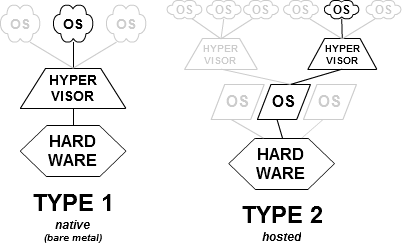
\includegraphics[scale=.8]{./pic/Hyperviseur.png}
    \caption{Different types of Hypervisors}
    \label{fig:Hypervisors}
\end{figure}

\subsection{Cloud Roles}
When cloud computing first started to take off, the main type of computing resource provided was IaaS in the public cloud \cite{sourcedigit}. This started to change in the recent years when two new types models for cloud computing emerged. Public and Hybrid clouds allowed for companies to utilize the power of the cloud while still having some or all of there resources located in their own data centers.

\subsection{Cloud Computing vs Standard Models}
The cloud computing environment has been growing quickly the last several years \cite{Vaquero}. However its important to understand the similarities and differences that this new type of computing brings. At the core cloud computing is no different then older client server models. The data is still on hard drives, servers still use OS environments, and networks still connect the servers to the Internet. The main difference between the two models is that in the cloud you pay for what you use and hardware configurations/problems are not a concern. Some of the advantages that cloud computing posses is the fact that there is rapid scalability. It is possible to spin up 100 machines and scale your service according to needs. There is also a level of abstraction between physical hardware and the systems. This provides a buffer, allowing for there to be problems with configurations, management, and physical hardware with little effect on the cloud hosted systems.

\subsection{Threats to the Cloud}
Cloud computing also has a different threat model compared to a normal dedicated server \cite{zissis2012addressing, mishra2013cloud, krutz2010cloud}. As cloud servers are, as the name suggests, in the cloud they usually will receive a pubic IP address that allows anyone to directly talk to them. This allows for direct communication to the running system which then exposes it to exploitation. The following list shows the potential attack vector's that a cloud computing systems has \cite{amini2015threat}.

\begin{itemize}
    \item In security data can be described in two ways, data at rest or data in transit. Data at rest is when data is stored on a system while data in transit is when data is moving between two destinations. If data can be accessed or read without the proper authentication it is then considered that a system has data loss.
    \item Account or service hijacking is when a unauthorized user is able to perform actions as another authenticated user. This may occur from insecurities with accounts or with insecurities revolving around authentication.
    \item For systems that are exposed to the Internet, an adversary may try to perform a denial of service attack on the system. This type of attack tries to overwhelm the system and not allow legitimate users to access the systems recourses.
    \item Data breaches occur when an unauthorized user is able to access sensitive data that is stored in databases. Database usually contain the most sensitive information that attackers can then sell. As cloud systems are typically accessible from the Internet, attackers attempt to probe security of systems to see if they can gain access to the back end databases.
    \item Abuse of cloud services Attackers also may use cloud systems to send spam or perform computationally intensive tasks (like BitCoin mining) for profit. They access a system via a vulnerability and then have scripts run that perform these tasks automatically.
\end{itemize}

\section{OpenStack}
OpenStack is an open source platform for cloud computing \cite{OpenStack}. OpenStack is built of many components that are designed to provide a different set of services (Nova, Neutron, etc.) the full list can be found on the open stack website located \footnote{ \href{https://www.openstack.org/software/project-navigator/}{https://www.openstack.org/software/project-navigator/}}. OpenStack is very scalable and diverse system that can be arranged to fit the needs of any cloud environment. For this project we ran OpenStack newton version 15.0.0.0.rc1. OpenStack is very modular with several core features running as the backbone of the software. The features that were used for this project were: Nova, Neutron, and Swift.

Nova is the service that provides access to OpenStack compute resources. It is the base service that a user would interact with the set up, run, configure, and destroy machines. Neutron is the service that controls and configures all of the networking between machines and the external network. This interlinks the Nova instances with the physical networking infrastructure.  Swift is the platform that is used for object and blob storage. It provides a large space for images, snapshots, and other storage needs to be assigned to.

One of the main aspects of OpenStack is a tool called Heat \cite{HeatOS}. Heat is a orchestration tool that setup environments though a script file. As the script file is read recourses, such as servers, floating IP addresses, and security groups are created. This tool allows complicated environments to be easily set up and deployed with little hassle for the administrator's. A community has been created to publish these helpful scripts. This leaves a problem as people use the scripts that are posted without full knowledge of what is happening in there environment. This may lead to services and machines exposed to the Internet without the user knowing about them.
\begin{figure}[H]
    \centering
    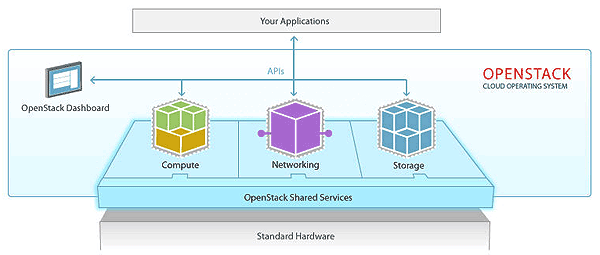
\includegraphics[scale=.6]{./pic/openstack-sm.png}
    \label{fig:OpenStack}
    \caption{OpenStack Cloud System}
\end{figure}

\section{SNIC Science Cloud}
At Uppsala University there is an OpenStack deployment on the UPPMAX super computer. This is allows professors and students to utilize cloud recourses for projects and courses.  This is a collaboration project under the Swedish National Infrastructure for Computing (SNIC) title.  This collaboration is between several institutions to provide large scale cloud recourses computation recourses to academia.

\section{Security}
The general focus of computer security is to ensure that computer systems follow the CIA model of confidentiality, integrity, and availability\cite{ComputerSecurity}. "The design artifacts that describe how the security controls (security countermeasures) are positioned, and how they relate to the overall IT Architecture. These controls serve the purpose to maintain the system's quality attributes, among them confidentiality, integrity, availability, accountability and assurance." \cite{it_security_architecture}. The disciplines that are focused on in this paper include: intrusion detection systems, network security, and system security.
Intrusion detection systems come in two main forms, host based and network based. A host based system runs on the host and attempts to detect any security threats on the host machine. A network based IDS is connected on the network and inspects network traffic, trying to find threats by inspecting network traffic patterns. Both of these systems have advantages and disadvantages. With a host based system software must be installed and configured on each system. In a network IDS system the packets are monitored for unusual traffic patterns. There are disadvantages to this type of solution also, mainly network traffic can be encrypted and the overall volume of traffic encountered. Some examples of network based IDS tools are \href{https://www.snort.org/}{Snort}.
A large portion of the problem for computer security comes from the networks that computers are attached to. The network allows other computers to communicate and attempt to access the particular machine. This is greatly increased if the computer is not placed behind a firewall/rougher and is directly accessible form the Internet. If an Internet facing computer is not updated properly vulnerabilities can be used to run unintended programs.
A unintended program running on a systems can be a concern. These programs can be used to send email spam, steal credentials, or participate in larger network attacks.

%For a cloud system where machines are provisioned and destroy setting up this type of system would be difficult. There for a network based IDS system was chosen.

\subsection{Network Security}
Network security aims to ensure that the underlying communication between hosts is secure. That may be to ensure that messages passed through the network are untampered or intercepted, ensure a device is properly protected from attach, or to divert/stop an attach reaching a machine. As this is a large field in itself we will break it down into smaller sections. Computers need to communicate with each other to relay information, this is done though the networking layers \cite{wiki:osiModel}. An attacker could, using different methods, intercept traffic and/or manipulate it. Network security in this context relates to ensure that information is preserved while in transit. For cloud security this type of network security is important to ensure that communication from a user to the machine is kept secure. Network security is also meant to protect machines from external network threats. This usually is done through a network firewall, which will sit between a external and internal network allowing only certain \"trusted\" traffic through. As most cloud machines are through some way exposed to the wide interest ensuring that traffic to the machines is trusted can be difficult. Most cloud based machines are operated through ssh and may need other ports open to communicate with other services or machines. This posses a network security problem as external open ports will be repeatedly attached by botnets \cite{wiki:botnets}. The last layer of security that the network can provide is protection against flooding or distributed denial of service attacks (DDOS attacks). These attacks try and overwhelm a server and take the service off line.

\subsection{System Level Security}
System security aims to protect running systems from malicious code execution. A malicious program is typically comprised of 2 pieces, an exploit and a payload. An exploit is a small mechanism designed to gain access to the system. Once access is gained the payload will be retrieved and executed. The payload then will perform actions like, lock file, upload user data, or capture keystrokes. Protection against this type of attack is mainly done though a host based intrusion detection system (HIDS) these are typically known as anti-virus or anti-malware. A HIDS is a small program that runs on a system scanning memory, disk, running processes, etc. If one of those matches a predefined rule then that code is quarantined and removed. These type of rule based systems lack in one particular area, they are bad at detecting new threats until a rule is created. Therefor newer HIDS try and use some type of machine learning or prediction to assert weather malicious code is being executed. Typically a security system will be set up on individual computers or servers. It will then run in the background protecting the system. In cloud security HIDS are a problem \cite(modi2013survey) as a wide variety of VMs may be created with users not knowing how to properly set up systems. Users may not know how to set up HIDS systems on these machines or the OS versions may not even support a HIDS.

\subsection{User Level Security}
User level security how reliant on how well users understand threats and access risks \cite{stanton2005analysis}. As users are the main proprietor of systems they hold the keys to ensuring that a system is safe from malicious adversaries. It however is problematic as many users don't understand system security and are not interested in learning it. The users then perform actions that compromise system security such as using weak passwords, opening ports to the Internet, and running unknown programs.

\subsection{Cloud Security Risks}
Cloud security posses several risk that are different from what a typical server might encounter. As all of the cloud systems are orchestrated and deployed via a web page there is a possibility of account takeover. This would allow an adversary to deploy machines with their own private keys that they would then be able to access. Deployed machines are usually orchestrated and created by users and not teams of administrator's. The user may not have the knowledge in secure computing, thus the system may be deployed in an insecure manner.

\section{User Recommendation}
The first stage of this project involved setting up user recommendations for configuring a secure VM and understanding some security features in the OpenStack platform. This involved taking the two main problems that the SNIC team faced: poorly secured SSH access and open ports. For starters the recommendation describes shat SSH is and how to use proper key pair authentication. The guild then goes onto describing ports and how to configure good security rules in OpenStack to prevent exposed ports. Below is a shortened list while the full readme can be found in the appendix.

\begin{itemize}
    \item ssh is the mechanism in which one should connect to cloud systems. It is a set of tools and protocols set to help ensure a secure connection between ones computer and server.
    \item A proper ssh key pair should be used. The key should be at least 2048 bits long and should have a password on it. This will ensure that even if the key is compromised no one would be able to use the key to get into any systems. One should never use user name and password authentication over ssh. There are a lot of bots on the Internet that attempt to break into systems that have week user name and password combinations in ssh.
    \item Once a key pair is created and the key is uploaded the private key should be securely held on the users computer.
    \item On the OpenStack side, users should use correct security groups for their machines. A security group is a way to define what ports a VM can access or be accessed by. This helps prevent unwanted exposure to ports on the machines.
    \item One should be aware of what services are run on each VM. These services may have open ports that enlarge the attack surface of the VM. These should either be turned off or the port should be blocked or filtered using the local firewall on the computer.
    \item Users of VMs should have a security mindset. This will greatly lower any potential vulnerabilities and is one of the best wes to prevent system compromise.

\end{itemize}

\section{Design Implementation}
A key part of this project was to create a simplistic interface that would allow an administrator to view changes to the environment and query for more information. Some base goals were created: scalability, ease of use, and intuitiveness. As the system is designed to be deployed over several cloud groups we needed a messaging system that could handle such a task. Email was first considered however it was soon realized that email would not work well due to the frequency of data sent and then inability to interact with the service. The next consideration was Internet Relay Chat (IRC), however as IRC is relatively unused in the professional work environment and users would need to learn how to interact with the protocol that idea was abandoned. Therefor as a final solution it was decided to work to build the messaging solution using Slack. This matched all of our starting criteria and allowed for a clean and simple implementation. Slack is a messaging application that allows groups of users to interact with one another in channels or directly. Once of the really neat features of this is the ability to program bots for users to interact with. Therefor the decision was made to create a bot that would interact with a channel for each cluster of machines. The bot would update the channel with any new information that the scan found ensuring that a constant flow was preserved. Users are also able to query to bot directly and get more information about the environment. This allows seamless integration between getting information from the environment and being able to dive deeper and investigate a machine.

For the first part of the project a modular design was created to enable further types of scanning to be added. An important aspect when designing the "watchdog" system with as little privileges as possible to prevent any unnecessary security holes. The watchdog is a phrase that was used throughout the project to describe the machine that performed all of the scanning. The following is a diagram of an example cloud environment.

\begin{figure}[H]
    \centering
    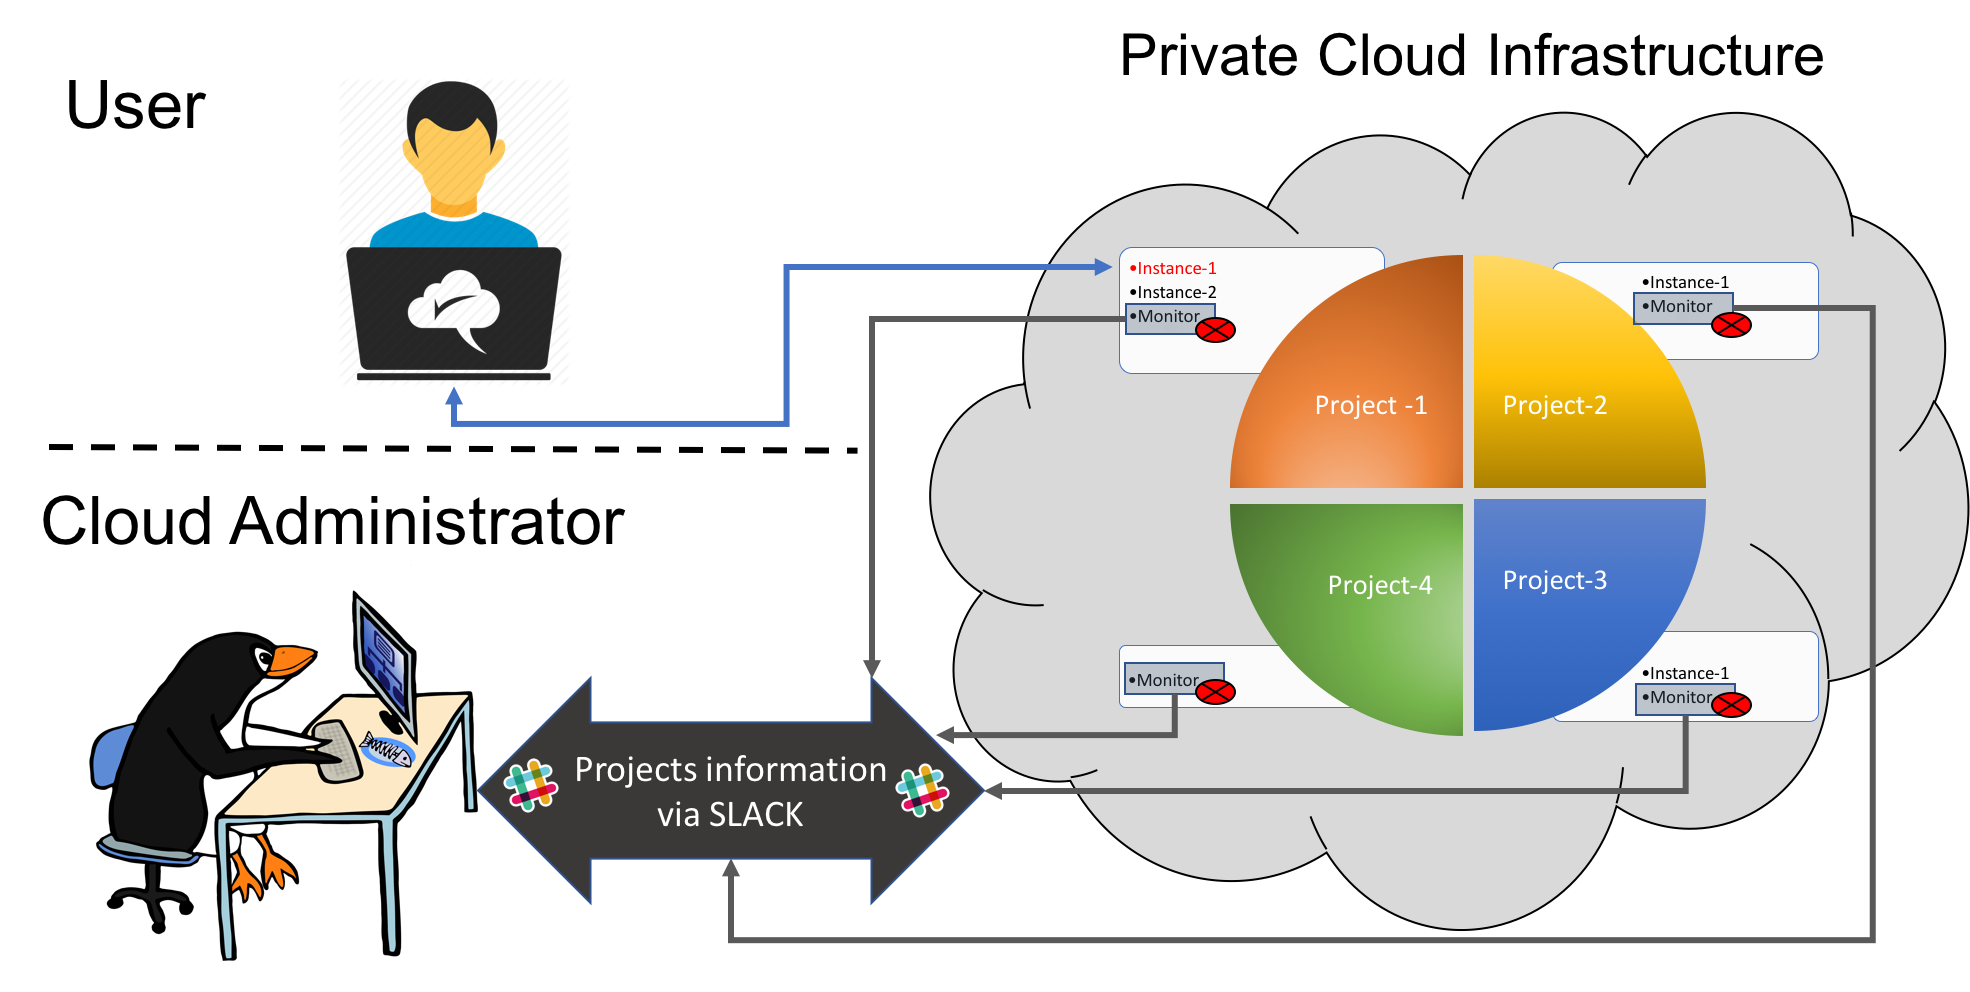
\includegraphics[scale=.4]{./pic/Picture1.png}
\end{figure}

The "watchdog" is initiated in the cloud cluster. The once initiated the VM will connect to the OpneStack Control Plain and get the list of servers, IP's, and floating IP's. Once that information is retreated the different modules will be run. In this standard case the two modules created were for nmap and ssh\_scan. Nmap is a tool used to scan a local or external network nd view what machines are funning on it. Nmap will be able to scan the machines ports and tell which ones are open and what services are running on them. It will also try and guess heuristically the operating system that is being run on the machine. This tool is therefor used in this system to find machines that have open ports and to see what services are run on them. If a service or port is found to not follow the recommendation then the VM can be terminated. The ssh\_scan tool is used to ensure that only a public private key pair are used. It will scan port 22 and alert if any other form of authentication is used.
These modules will gather the results from the network and collect them into a central repository. Once the data is gathered it is compared to the config file.  If a discrepancy is found between the expected results and the scanned machine is found an alert is sent to the administrator. For this project the administrator receives notification on a separate slack. This entire process is run every 20 min by a corn job located on the watchdog machine. This type of design allows for a flexible platform that can have each component further customized.

\section{Architecture}
For the monitoring resource an important architecture design was to ensure that the system was modular.  This enabled the system to be adapted to different cloud environments. Users would be able to create individual monitoring tools or logging techniques to be used for configuring to specific infrastructures. As for the proof of concept project Nmap and ssh\_scan were implemented.

The main portion of the entire program is the database. As the system is designed in a modular manner all the data is stored and retrieved from the database. The database is a MongoDB instance that has one collection that hold all the data from different scans. The only data that is needed inside of the database is the server ID\@. This is the key to which all other data about a particular machine is added to. When data is stored the ID of the VM is passed along with the data. When a user requests data they must also provides the ID for the data they would like.

Apart from the database the other modules are started from the main python program. To do this the system will first connect to the OpenStack backend via credentials provided in a configuration file. This will pull down all of the VM IDs. This is then feed to each scanning model. These modules intern can query the backend for any additional information that they need. To illustrate this the Nmap modules will use the provided IDs to obtain the internal and external IP address for each machine. This will then feed the query to the Nmap program. The Nmap model will then obtain the data and parse out the needed information, such as open ports. Once the data from the model is as wanted it will be sent to the database to be added for each VM.

To add a new model the main function must be edited so that it will call the new model. The output from the new model must follow a set standardized of $(ID: "ID number", data)$ this is then sent via the main function to the database model to be interested into the database.

The Slack bot uses the slack API to communicate with the Slack web interface. The API allows for messages to be sent between the bot and the Slack servers.

\begin{figure}[ht]
    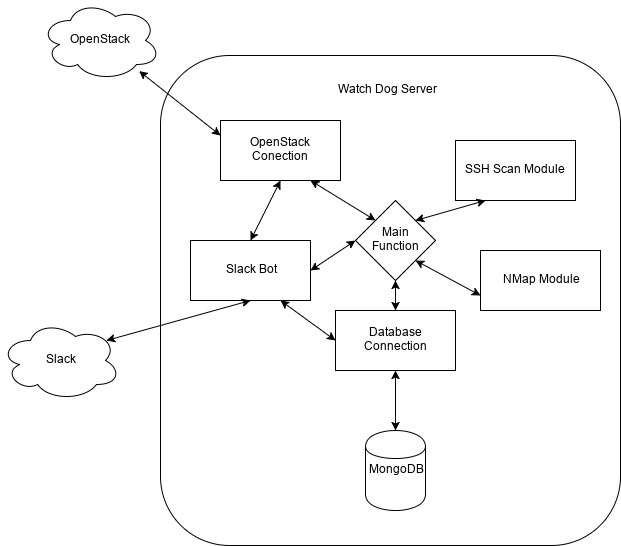
\includegraphics[scale=.5]{./pic/Arcitecture.png}
    \caption{Intrusion detection system architecture, the main component is the "Main Function" and the database. All information is feed through the main function allowing fetures to easly be interchanged and expanded.}
\end{figure}

\newpage

\subsection{Tools}
For this project there were several external tools that were used. These tools were picked to perform specific tasks like collect ssh configuration data.

\subsubsection{Nmap - Network Scanning Tool}
Nmap is a network scanning solution that can be used to scan for open ports, running services, network topography, and others \footnote{\href{https://nmap.org/}{https://nmap.org/}}. Nmap allows for scanned data to be saved into an \.xml file that can then be filtered and input into the database.

\subsubsection{ssh\_scan - SSH Security Auditing Tool}
Ssh\_scan is another tool used to gather information about remote ssh configurations. It is able to detect the type of authentication, ssh protocol used, and several others \footnote{\href{https://github.com/mozilla/ssh\_scan}{https://github.com/mozilla/ssh\_scan}}. The output is saved to a json file that is then read into the database.

\subsubsection{Slack Bot}
Slack bot is a small bot built on top of the Slack api to display information form the database and query data in real time. The bot will connect to a channel specifically created for each cloud cluster. There the bot will print relevant information from the database. One of the advantages that Slack provides is the ability to communicate between the users and the bots. Users are also able to query the database via the bot, this allows an administrator to quickly find a problem and find information about that machine with ease.

\subsubsection{Ansible - Sever Orchestration Tool}
Ansible is a tool designed to automate system deployment. The tool has a scripting language that describes steps for systems to be configured.
\begin{mdframed}
\begin{lstlisting}
---
- hosts: all
  remote_user: ubuntu
  gather_facts: no
  pre_tasks:
    - name: Update and install python
      with_items:
        - python
        - python-dev
        - python-setuptools
        - git-core
        - gcc
        - nmap
        - ruby
        - ruby-dev
        - libsqlite3-dev
        - make
        - htop
        - nload
        - mongodb-org
        - sqlite3

\end{lstlisting}
\end{mdframed}

In the above example for all hosts in a separate host file the system will login as "ubuntu" and install the list of programs using $apt-get$. The default connection ot each host is done via SSH where the user points the ansible program to their private key.  This tool is used to deploy complex environments with little hassle.  As this project was also designed to be easily deployed ansible was chosen. There are several other tools such as Puppet or Chef. However prior knowledge and usability determined the software chose.

\subsubsection{Git - Source Control}
An important tool used throughout this project was git. Git is a version control system that keeps track of all changes to files. In addition it allows for uploading of these changes to websites like GitHub\footnote{\href{https://www.github.com}{https://www.github.com}} and Bitbucket \footnote{\href{https://www.bitbucket.org}{https://www.bitbucket.org}}. This creates a viewable time line of all changes to the code base as well as provides a backup in the cloud in case of a system failure.

\section{System Interaction}
One of the important aspects of the system that was create was intractability. We wanted to present the administrator with a tool that would allow them to gain all the information that they wanted about a system. We wanted the user to be able to intact with a bot, and have the bot respond with the relevant information that the user wanted. The system should be fluid and informative, without the user having to switch between different programs to find relevant information. To communicate with the bot, the user simply calls the bot using the $@$ sign and then the command.

The picture bellow show the help command.
\begin{figure}[H]
    \begin{mdframed}
    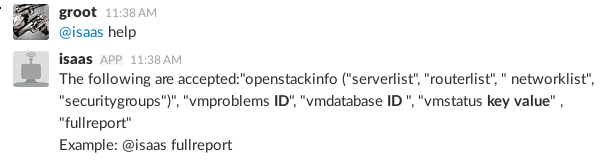
\includegraphics[scale=.5]{./pic/2017-06-26-113851_606x161_scrot.png}
    \end{mdframed}
\end{figure}

The picture below shows how a full report for a project can be generated.
\begin{figure}[H]
    \begin{mdframed}
    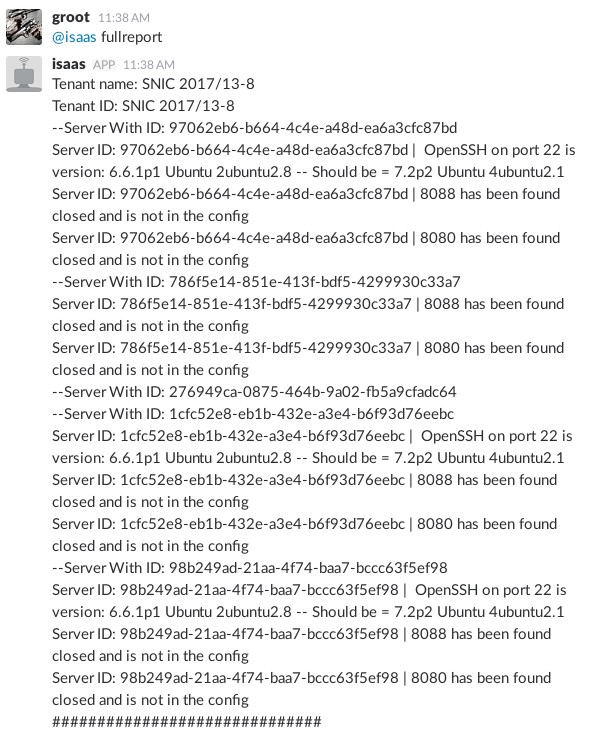
\includegraphics[scale=.5]{./pic/2017-06-26-113829_608x740_scrot.png}
    \end{mdframed}
\end{figure}

The picture below shows how to call another bot and retrieve a projects router information.
\begin{figure}[H]
    \begin{mdframed}
    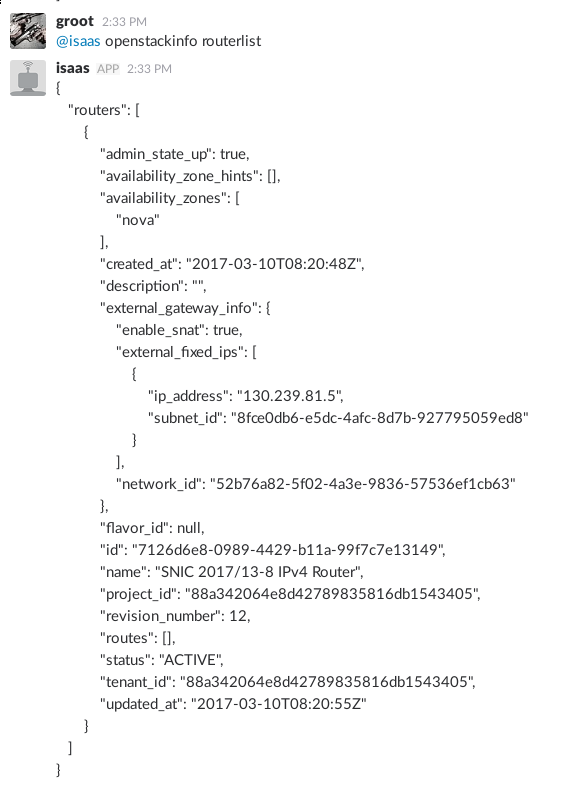
\includegraphics[scale=.5]{./pic/2017-06-26-113808_563x789_scrot.png}
    \end{mdframed}
\end{figure}

\section{Tests}
The system was designed and created in a testing environment. The environment was hosted in an OpenStack cloud environment with several test vms initiated. The $watchdog vm$ was then spun up and the code was deployed. The code was then edited and redeployed via Ansible. New features were able to be tested on a live deployment ensuring that when deployed to other clusters they would function as needed. To ensure that the code functioned with little bugs, tests were run by spinning up new vms and changing there configurations.

\section{Results}

\subsection{User Recommendation}
A user recommendation was written to help users properly connect to initialized VMs. The recommendation focuses on how to connect to the VMs using a proper ssh key. The guild first walks thought how to set up a ssh key pair on a users local machine. This ensures that a user creates a proper strong key pair. The user is then instructed on how to add the public key to the OpenStack interface. Along with the ssh connection other simple recommendations are provided to the user. These are to help a user understand the different security implications no mater what they use the VM for. Some examples of what the recommendations looks at are, open ports and security rules. The user recommendation can be found at the following url \footnote{\href{https://github.com/DarkLog1x/MasterThesis/tree/master/UserRecomendation}{https://github.com/DarkLog1x/MasterThesis/tree/master/UserRecomendation}}

\subsection{Intrusion Detection System Results}
The administrators first create a configuration file for the cloud system. This configuration file is set for the system to know what type of system configuration the servers should have. Below is a typical configuration:

\begin{mdframed}
    \begin{lstlisting}
#This is a config file
#It needs to be filled out similer to the output of the script that is run (a.k.a - NMAP, ssh_scan, etc)
#* special case to print all other open port
ports: 22 - open
ports: 80 - closed
ports: 443 - closed
ports: 5000 - closed
ports: 6000 - closed
IP: ip_external_auth - publickey
IP: ip_internal_auth - publickey
    \end{lstlisting}
\end{mdframed}
The file is read in line by line. All lines that start with a \# are comments and are ignored. The system will then parse each line, splitting each line via the $:$ and $-$ character. The system then uses the split line to view the type of scan that command is associated to, the information to look for, and then the expected result. If the result does not match the output the output is flagged and sent to the communication mechanism, in this case Slack.

Once the base system was running in our test environment a decision to scale up was made. Our test environment was compatible however a real environment with more machines and users could not have been replicated. Luckily a class was taking place that used the cloud environment. Therefor a watchdog vm was spun up in the classes cloud cluster and started to monitor the vms that were created. Immediately vms started to appear in the Slack channel. After running for a while inconsistencies were started to be found. A small snippet of the Slack channel is shown bellow. In this section 5 machines are shown, 3 of them have inconsistencies that are not in the configuration file.

The following table describes how the output of the Slack bot will look like.

\begin{table}[H]
\centering
\caption{Slack Ouput Breakdown}
\label{Slack Ouput Breakdown}
\resizebox{\textwidth}{!}{%
\begin{tabular}{|p{2cm}|p{6cm}|p{8cm}|}
\hline
\rowcolor[HTML]{C0C0C0}
Line Number & VM ID & Description \\ \hline
1.            &  930ee1bb-e07a-461f-b09f-1e1a9c864a36     & There are 3 open ports (lines 2-4) that should be closed.  \\ \hline
5.            &  f57b9369-4e15-4151-9b0b-7d405cbdb5e4     & The VM allows for user authentication via a username and password.            \\ \hline
10.            &  81933a08-9451-4d16-aca4-9fb6269b4e0d     & There are 3 open ports (lines 2-4) that should be closed.            \\ \hline
9. and 14. &  ad74be2b-e452-43df-b307-d8ad3bcd6cb7 and  6e19b2a1-1dbd-4fe1-83d6-8e57cdd08ff7    & The VMs are running and follow the configuration.             \\ \hline
\end{tabular}
}
\end{table}

\begin{mdframed}
\begin{lstlisting}
 1.   --Server With ID: 930ee1bb-e07a-461f-b09f-1e1a9c864a36
 2.   Server ID: 930ee1bb-e07a-461f-b09f-1e1a9c864a36 | 8088 has been found open and is not in the config
 3.   Server ID: 930ee1bb-e07a-461f-b09f-1e1a9c864a36 | 8042 has been found open and is not in the config
 4.   Server ID: 930ee1bb-e07a-461f-b09f-1e1a9c864a36 | 8031 has been found open and is not in the config
 5.   --Server With ID: f57b9369-4e15-4151-9b0b-7d405cbdb5e4
 6.   Server ID: f57b9369-4e15-4151-9b0b-7d405cbdb5e4 |  ip_external_auth: publickey password keyboard-interactive -- Should be = publickey
 7.   Server ID: f57b9369-4e15-4151-9b0b-7d405cbdb5e4 |  ip_internal_auth: publickey password keyboard-interactive -- Should be = publickey
 8.   Server ID: f57b9369-4e15-4151-9b0b-7d405cbdb5e4 |  OpenSSH on port 22 is version: 7.4 -- Should be = 7.2p2 Ubuntu 4ubuntu2.1
 9.   --Server With ID: ad74be2b-e452-43df-b307-d8ad3bcd6cb7
 10.   --Server With ID: 81933a08-9451-4d16-aca4-9fb6269b4e0d
 11.   Server ID: 81933a08-9451-4d16-aca4-9fb6269b4e0d | 8088 has been found open and is not in the config
 12.   Server ID: 81933a08-9451-4d16-aca4-9fb6269b4e0d | 8042 has been found open and is not in the config
 13.   Server ID: 81933a08-9451-4d16-aca4-9fb6269b4e0d | 8031 has been found open and is not in the config
 14.   --Server With ID: 6e19b2a1-1dbd-4fe1-83d6-8e57cdd08ff7
\end{lstlisting}
\end{mdframed}

Once a potential problem was found the \emph[bot] can be queried to get a full report of the virtual machine in question.

\begin{figure}
\begin{mdframed}
\begin{lstlisting}
    Tenant name: SNIC 2017/13-8

    Tenant ID: SNIC 2017/13-8

    [
    {
        "ID": "f57b9369-4e15-4151-9b0b-7d405cbdb5e4",
        "IP": {
            "ip_external": "130.239.81.28",
            "ip_external_auth": "publickey password keyboard-interactive",
            "ip_internal": "192.168.1.9",
            "ip_internal_auth": "publickey password keyboard-interactive"
        },
        "OpenStack_info": {
            "created_at": "2017-03-16T08:09:08Z",
            "image_id": "e4752852-c053-4fee-b198-6d990d914e3a",
            "image_name": "CoreOS - latest",
            "updated_at": "2017-03-16T08:09:25Z",
            "user_id": "d152c3dbd72c44af95ac4e6e48ccb0ec"
        },
        "_id": {
            "\$oid": "58db779eb39aa86565e2f1f3"
        },
        "ports": {
            "22": "open"
        },
        "services": {
            "OpenSSH on port 22 is version": "7.4"
        }
    }
    ]
\end{lstlisting}
\end{mdframed}
\end{figure}

The administrate then gets a full view of the machine in question and can then decide what the best possible next action is. As mentioned before the type of data that is present is not fixed therefor each module would add its own collected data for each specific VM. Therefor only the relevant data for the machine is displayed. This type of information condensed information was not present before this system wad developed. Administrators would need to run several programs to gather the data and then would need to synthesis it by hand.

\subsection{Hypervisor Information Gathering Results}
Once a compromised machine has been found a copy of the memory, disk, and system information is made. This is to help if the administrators would like to further understand what happened. To do this a script was written that uses the \lstinline{virsh} tool to connect to the kvm. Once connected the script pull relevant data and stores them into temporary files.

The data that the script pulled is a disk image, the memory of the machine, and the cpu state. The disk image saves the state of the hard drive and allows for the machine to be recreated if need be. The memory is saved as a raw memory dump. This creates a large file that represents the active memory from the virtual machine. Lastly the cpu state is saved to show the cpu usage. These 3 items provide a comprehensive overview of what the machine was doing at the time. This would then allow an administrator to further figure out the cause of the exploit. The administrator could use tools like volatility framework \cite{volitilityFram} to then import the memory dump and then attempt to find what programs nad services were running on the machine.

\section{Discussion}
Throughout the project an attempt was made to ensure that the project was well designed and created. However due to time constraints the code portion of the project will be branded as a prototype. This is because there are several drawbacks that could not have been overcome in this specific time frame. The current implementation utilizes a individual VM for every cluster. This increases resources use quickly, if a cloud system had 100 clusters then there would be 100 VMs that would only be used for monitoring. It would be beneficial if it was possible to have a smaller number of VMs used to scan multiple clusters. However the current system is unable to perform this type of task. Currently Slack is used as a medium to communicate between the administrators and the scanning mechanism. This has proved to be an interesting tool allowing for bidirectional communication and quick information retrieval. However the reliance on Slack may be jeopardized if Slack decides to change their api's, limit bots, or goes out of business. Luckily the system was designed in such a way to allow any communication medium to be added to the system. Therefor if Slack does not continue to meet the standards that an organization needs another tool can be used to replace Slack with ease. Some alternatives to Slack could be HipChat or IRC.
An issue that was ran into later during the creation of the project was that the Slack channel would get cluttered if a lot of different devices were not following the configuration file. One way to sort out the higher risk targets would be to add symbol's. These symbol's would be able to indicate the severity level / risk that each output would pose. The severity level would have to be decided by the administrative team. Some ideas to fix this were thought of but were not implemented due to time constraints.

\section{Future Work}
The project has a large potential to be expanded. As the code written now is only a prototype there is more work that can be added to expand the tools usefulness. As the code is created with modularity in mind, a user can easily add new scans into the project. If a user wanted, for example, to ensure that a website is correctly configured they could add the nikto \cite{NiktoScan} vulnerability scanner. The scan can then be run and the data would be added to the database. Another future work that could be expanded on is allowing for different methods of interacting with the system. Currently Slack is used, however administrator's might want email reports or an IRC channel instead of Slack. Luckily this can easily be integrated and several systems can be used asynchronously. This allows for administrators to custom configure this system to their desired needs and specifications. In addition the project is opensource, therefore anyone is allowed to take the code and modify it. This allows for individuals to expand the project in whatever direction that they see fit.

\section{Conclusion}
As was shown the cloud environment is a complex tool that is steadily growing and innovating. These cloud recourses give users an incredibly powerful and flexible tool to create complex systems that are independent from hardware. As users gain full controls of systems directly connected to the Internet. System security becomes a user based, however as mentioned users may not know best practices therefor leaving systems vulnerable to compromise. With users and organizations switching over to using cloud resources in everyday situations new attack become ever more present. Many of the leaders in the public cloud have created proprietary solutions to attempt to protect thiere users and systems from compromise. However many of the private clouds using open source solutions, like OpenStack, may not have the recourses or knowledge to create such solutions. Therefore this project was designed and created to prototype a system that is able to actively scan private clouds for potential vulnerabilities. Administrators are able to see results and query an automated system for further information with ease. A lot was learned about the threat landscape of cloud systems and how a modular system can be designed. It is the hope of the author that this system can be used by other people to ensure that any private cloud environment is secure.


\newpage
\bibliographystyle{plain}
\bibliography{thesis.bib}
\newpage
\appendix
\section{}
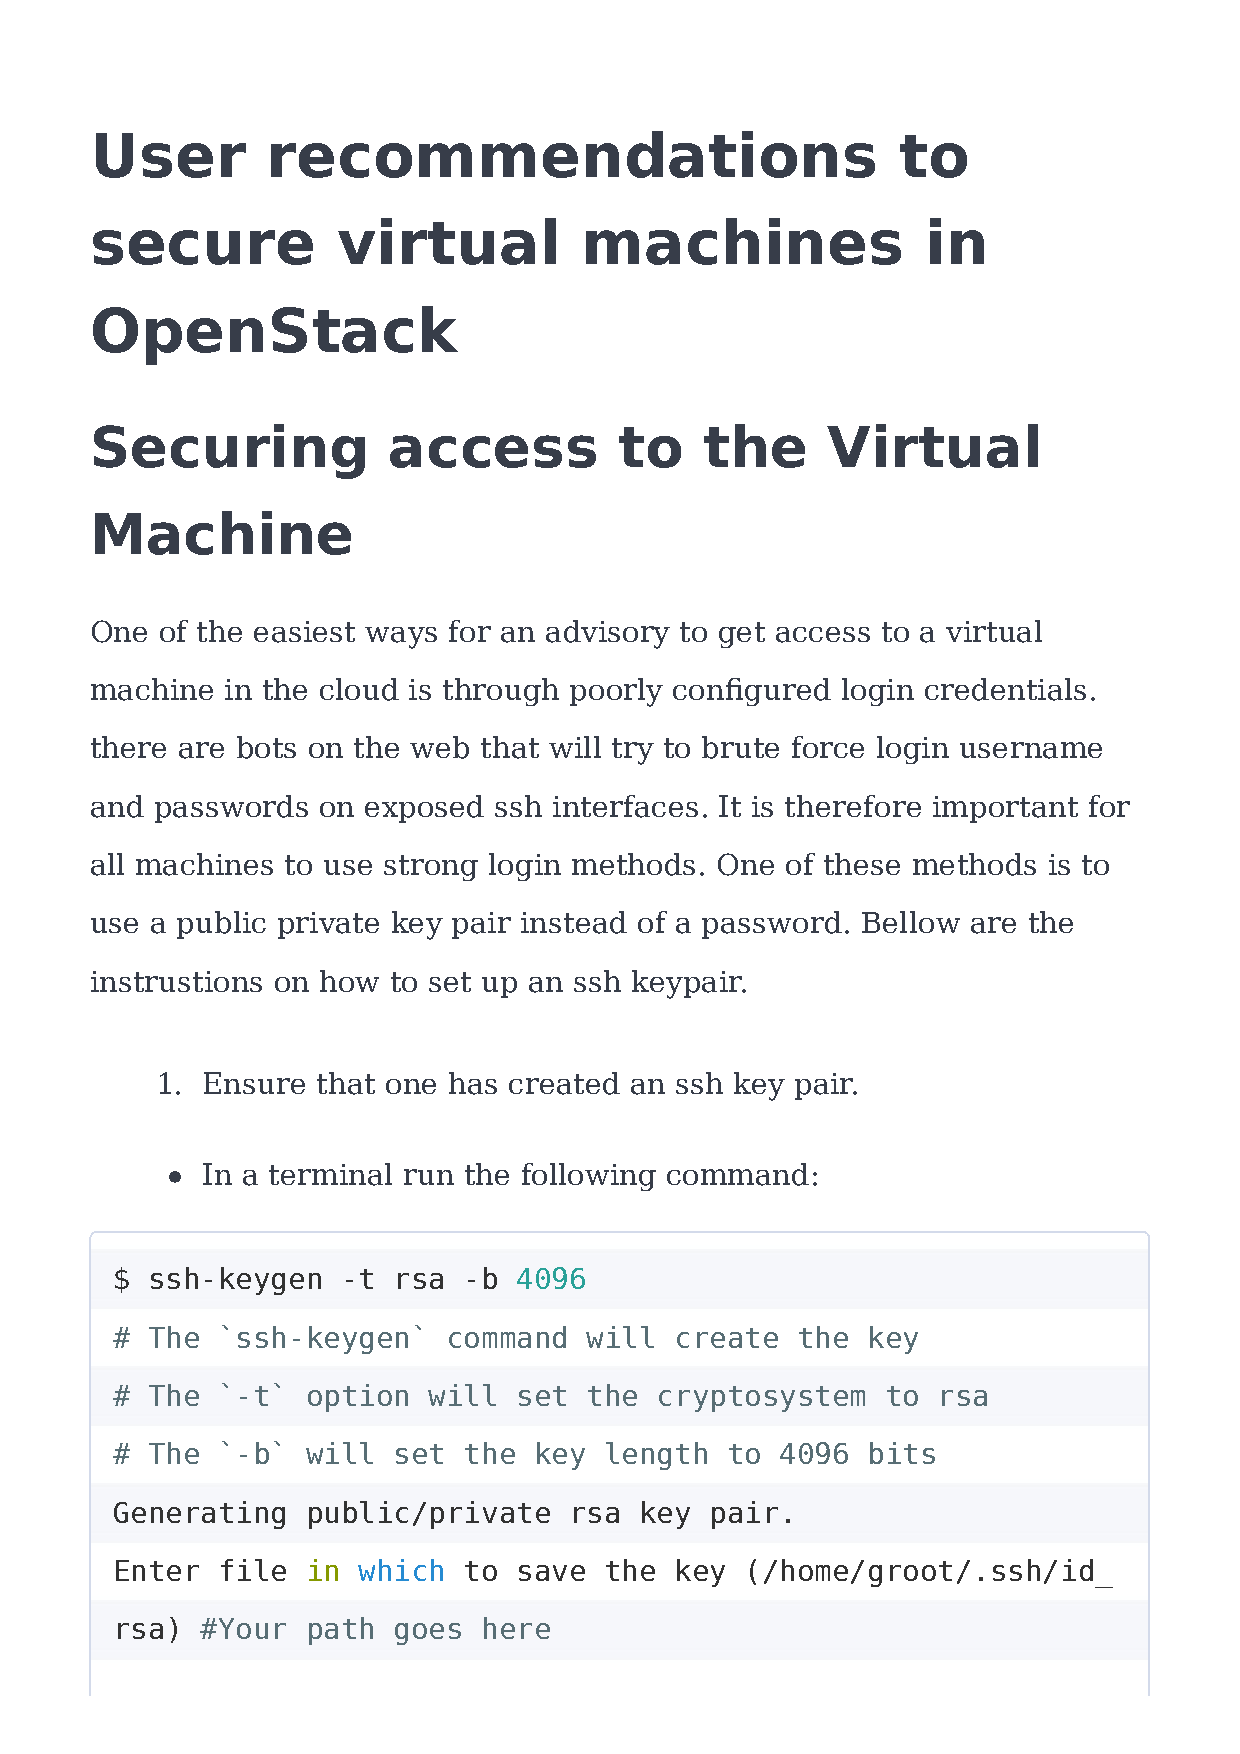
\includepdf[pages=-, scale=0.7]{README.pdf}
\end{document}
